\documentclass{article}
\usepackage{cmap}
\usepackage[utf8]{inputenc}
\usepackage[english,ukrainian]{babel}
\usepackage{graphicx}
\usepackage{geometry}
\usepackage{listings}
\usepackage{float}
\usepackage{amsmath}
\usepackage{subfig}
\geometry{
	a4paper,
	left=20mm,
	right=20mm,
	top=15mm,
	bottom=15mm,
}
\lstset{
	language=c,
	tabsize=4,
	keepspaces,
	showstringspaces=false,
}
\graphicspath{ {./pictures} }
\setlength{\parindent}{4em}

\newcommand\subject{Архітектура комп'ютера}
\newcommand\lecturer{доцент кафедри ПЗ\\Крук О.Г.}
\newcommand\teacher{доцент кафедри ПЗ\\Крук О.Г.}
\newcommand\mygroup{ПЗ-22}
\newcommand\lab{3}
\newcommand\theme{Моделювання та дослідження основних типів тригерів в СИСТЕМІ Proteus}
\newcommand\purpose{Закріпити практичні навики моделювання логічних схем в середовищі системи програм Proteus; поглибити знання про будову та функціонування основних типів тригерів; ввести їх схеми та виконати моделювання в системі програм Proteus; дослідити на основі отриманих часових діаграм їх роботу}

\begin{document}
\begin{normalsize}
	\begin{titlepage}
		\thispagestyle{empty}
		\begin{center}
			\textbf{МІНІСТЕРСТВО ОСВІТИ І НАУКИ УКРАЇНИ\\
				НАЦІОНАЛЬНИЙ УНІВЕРСИТЕТ "ЛЬВІВСЬКА ПОЛІТЕХНІКА"}
		\end{center}
		\begin{flushright}
			\textbf{ІКНІ}\\
			Кафедра \textbf{ПЗ}
		\end{flushright}
		\vspace{200pt}
		\begin{center}
			\textbf{ЗВІТ}\\
			\vspace{10pt}
			до лабораторної роботи № \lab\\
			\textbf{на тему}: “\textit{\theme}”\\
			\textbf{з дисципліни}: “\subject”
		\end{center}
		\vspace{112pt}
		\begin{flushright}
			
			\textbf{Лектор}:\\
			\lecturer\\
			\vspace{28pt}
			\textbf{Виконав}:\\
			
			студент групи \mygroup\\
			Коваленко Д.М.\\
			\vspace{28pt}
			\textbf{Прийняв}:\\
			
			\teacher\\
			
			\vspace{28pt}
			«\rule{1cm}{0.15mm}» \rule{1.5cm}{0.15mm} 2022 р.\\
			$\sum$ = \rule{1cm}{0.15mm}……………\\
			
		\end{flushright}
		\vspace{\fill}
		\begin{center}
			\textbf{Львів — 2022}
		\end{center}
	\end{titlepage}
		
	\begin{description}
		\item[Тема.] \theme.
		\item[Мета.] \purpose.
	\end{description}

	\section*{Індивідуальне завдання}
\begin{figure}[H]
		\centering
		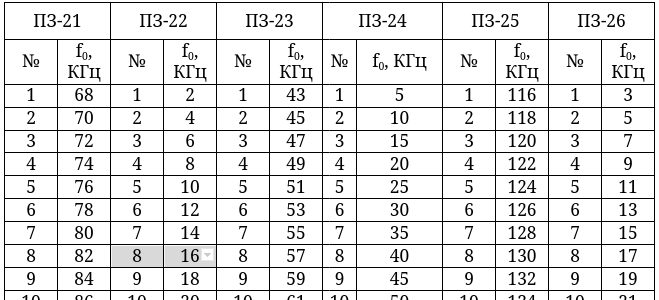
\includegraphics[scale=0.75]{v}
	\end{figure}	

	\section*{Теоретичні відомості}
	Тригер – це електронний вузол з двома стійкими станами, зміна яких відбувається під дією вхідних сигналів. Якщо прийняти один стан тригера за логічний нуль, а інший – за логічну одиницю, то виходить, що тригер є елементом пам’яті, який може зберігати один біт інформації. Тригер є найпростішим представником послідовнісних пристроїв і водночас обов’язковим елементом всіх функціонально закінчених вузлів і блоків.
	
	У послідовнісних пристроях (цифрових автоматах з пам’яттю або скінченних автоматах) вихідні сигнали в кожний момент часу залежать не лише від поточних значень на входах, але й від внутрішнього стану, який є наслідком попередніх дій вхідних сигналів. 
	
	На основі тригерів будують типові функціональні вузли комп’ютерів – регістри, лічильники, накопичувальні суматори, а також мікропрограмні автомати.
	
	Усі різновиди тригерів можна розглядати як елементарний автомат, що складається з власне елемента пам’яті (ЕП) та схеми керування (СхК), яка утворює вхідну логіку (рис. 3.1). Схема керування забезпечує записування, зчитування, стирання та індикацію двійкової інформації, яка зберігається в тригері. 
	
	
	\section*{Хід роботи}
	
	\section*{Схема 1}	
	\begin{figure}[H]
		\centering
		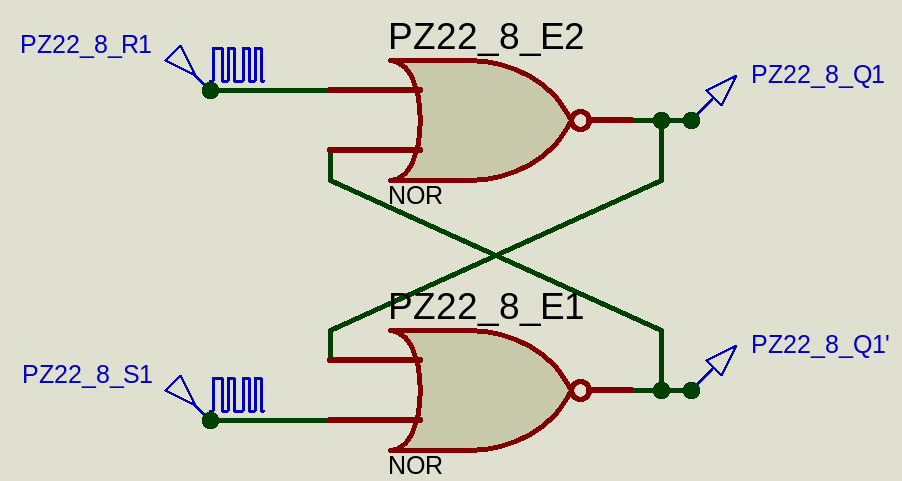
\includegraphics[scale=0.25]{s1}	
		\caption{Схема 1}
	\end{figure}

	\begin{figure}[H]
		\centering
		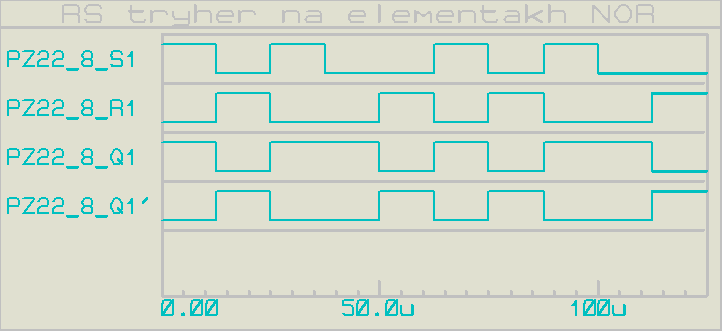
\includegraphics[scale=0.25]{g1}	
		\caption{Графік до схеми 1}
	\end{figure}
	
	\section*{Генератори до схеми 1}
	\begin{figure}[H]
		\centering
		\subfloat[]{{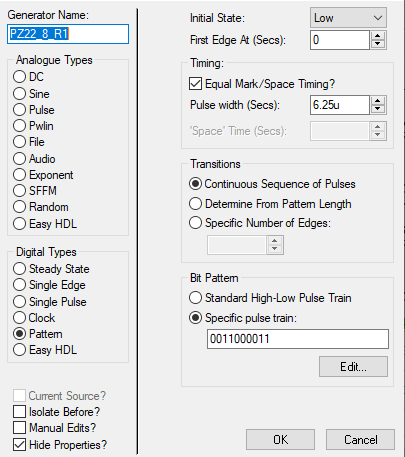
\includegraphics[width=0.45\textwidth]{11}}}
		\hspace{5px}
		\subfloat[]{{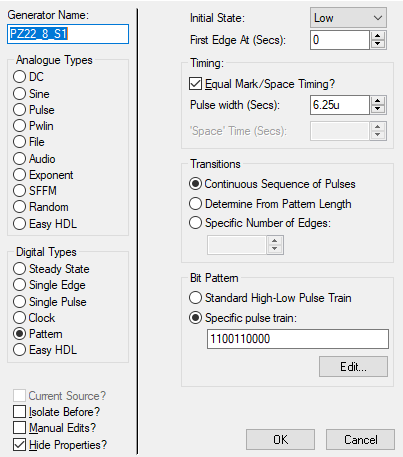
\includegraphics[width=0.45\textwidth]{12}}}
	\end{figure}

	\section*{Схема 2}	
	\begin{figure}[H]
		\centering
		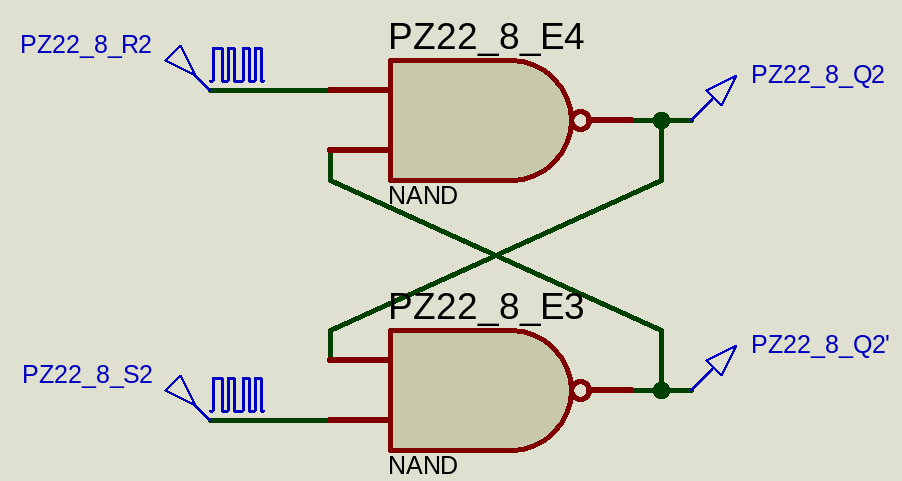
\includegraphics[scale=0.25]{s2}	
		\caption{Схема 2}
	\end{figure}
	
	\begin{figure}[H]
		\centering
		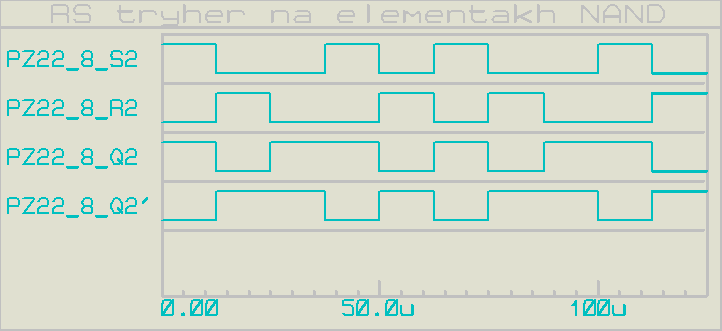
\includegraphics[scale=0.25]{g2}	
		\caption{Графік до схеми 2}
	\end{figure}

	\section*{Генератори до схеми 2}
	\begin{figure}[H]
		\centering
		\subfloat[ ]{{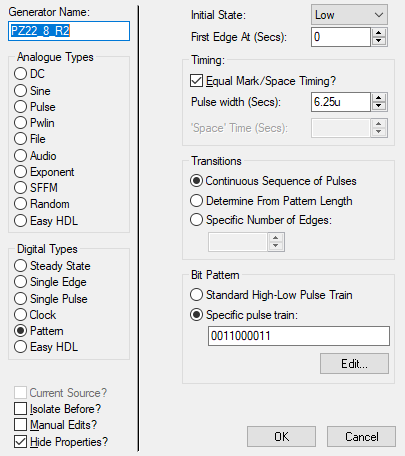
\includegraphics[width=0.45\textwidth]{21}}}
		\hspace{5px}
		\subfloat[ ]{{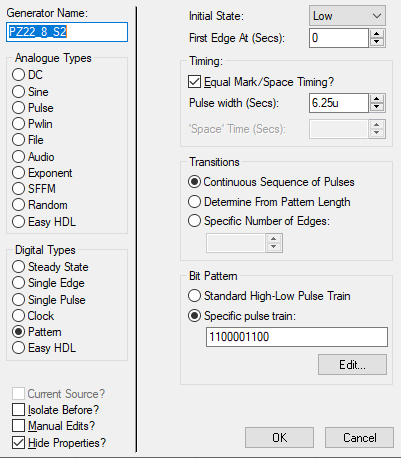
\includegraphics[width=0.45\textwidth]{22}}}
	\end{figure}

	\section*{Схема 3}	
	\begin{figure}[H]
		\centering
		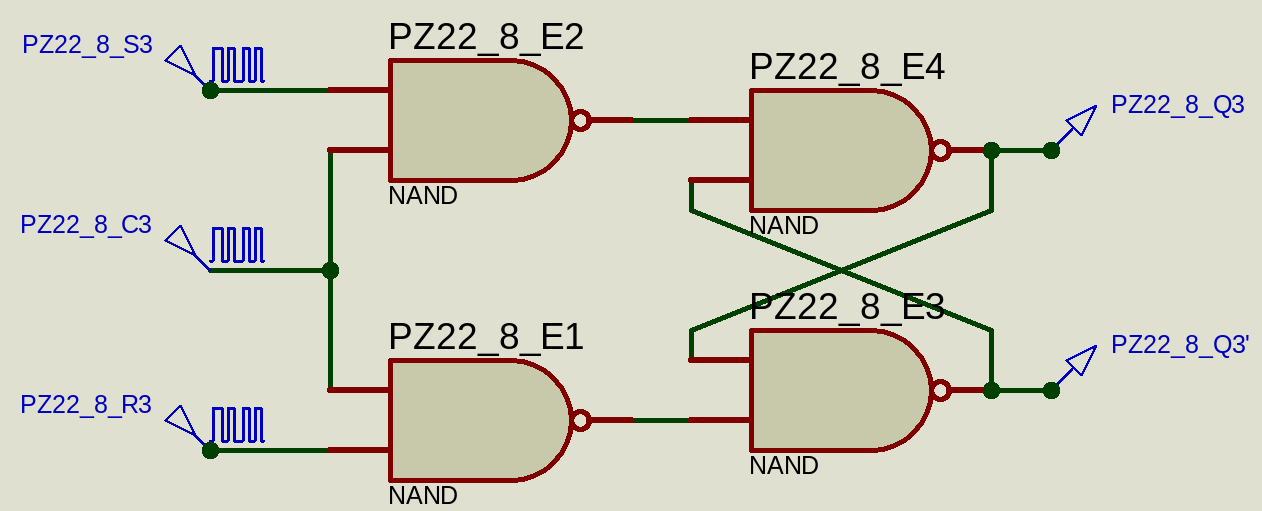
\includegraphics[scale=0.25]{s3}	
		\caption{Схема 3}
	\end{figure}
	
	\begin{figure}[H]
		\centering
		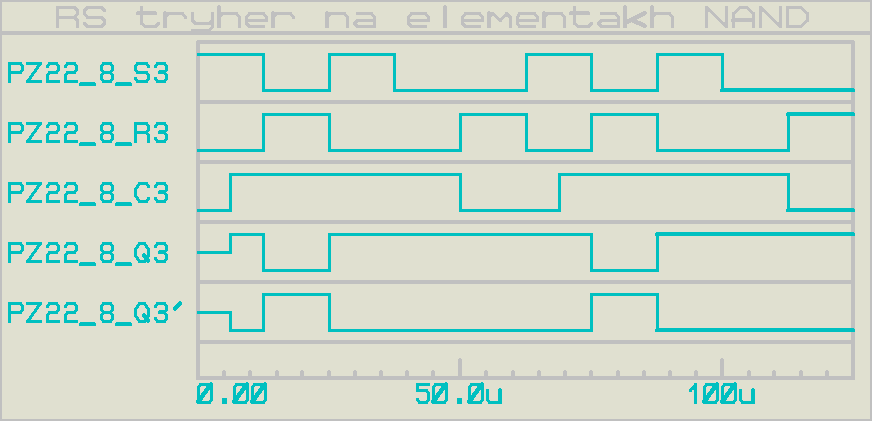
\includegraphics[scale=0.25]{g3}	
		\caption{Графік до схеми 3}
	\end{figure}

	\section*{Генератори до схеми 3}
	\begin{figure}[H]
		\centering
		\subfloat[ ]{{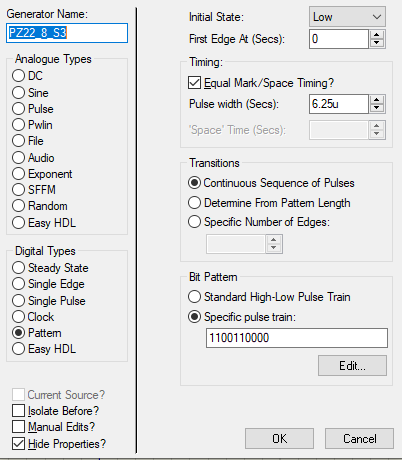
\includegraphics[width=0.45\textwidth]{31}}}
		\hspace{5px}
		\subfloat[ ]{{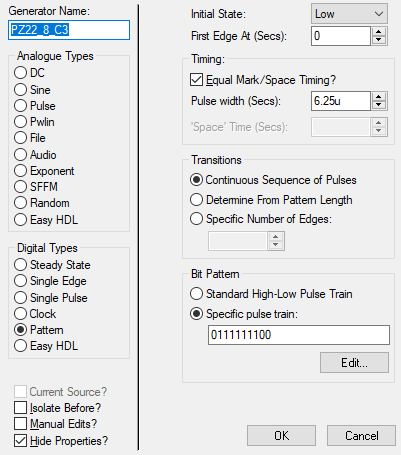
\includegraphics[width=0.45\textwidth]{32}}}
		
		\subfloat[ ]{{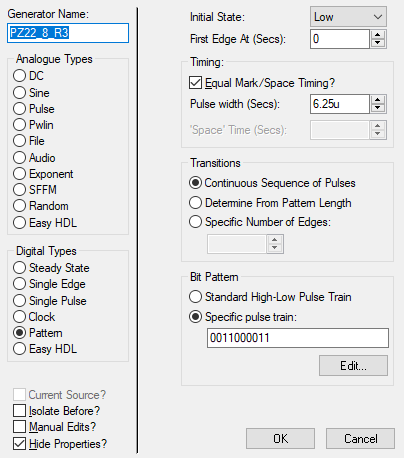
\includegraphics[width=0.45\textwidth]{33}}}
	\end{figure}

	\section*{Схема 4}	
	\begin{figure}[H]
		\centering
		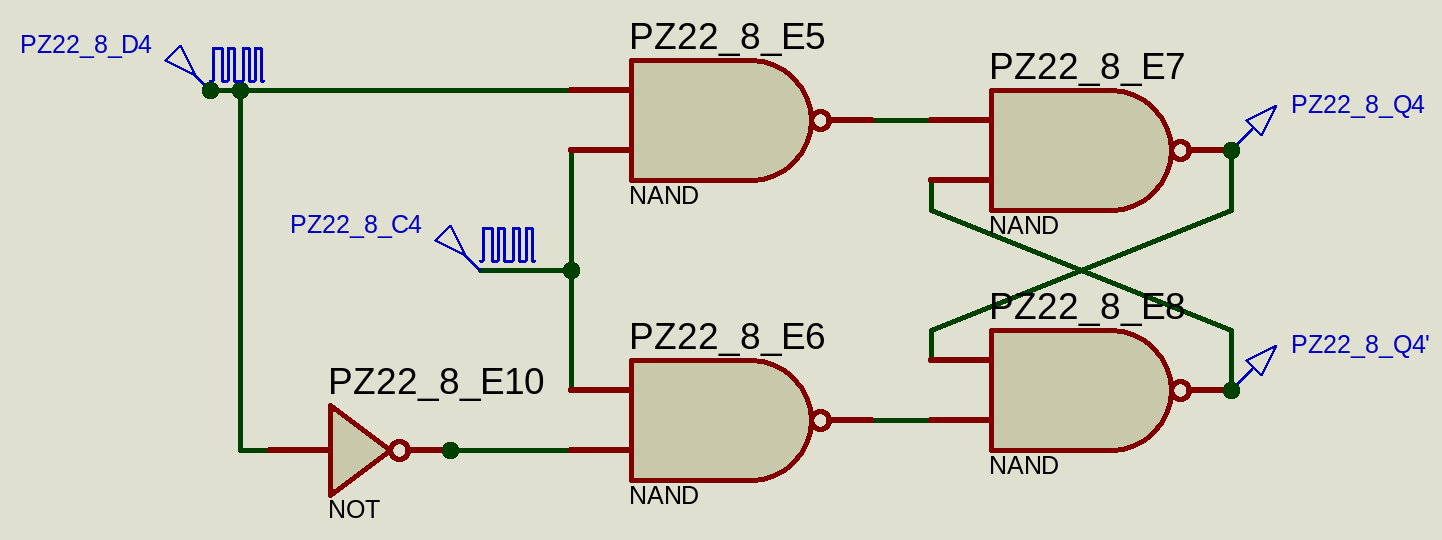
\includegraphics[scale=0.25]{s4}	
		\caption{Схема 4}
	\end{figure}
	
	\begin{figure}[H]
		\centering
		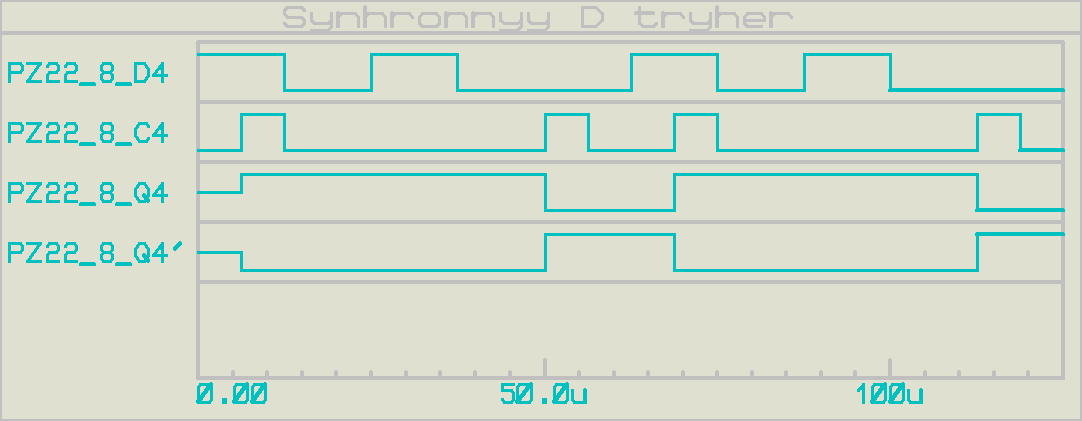
\includegraphics[scale=0.25]{g4}	
		\caption{Графік до схеми 4}
	\end{figure}

	\section*{Генератори до схеми 4}
	\begin{figure}[H]
		\centering
		\subfloat[ ]{{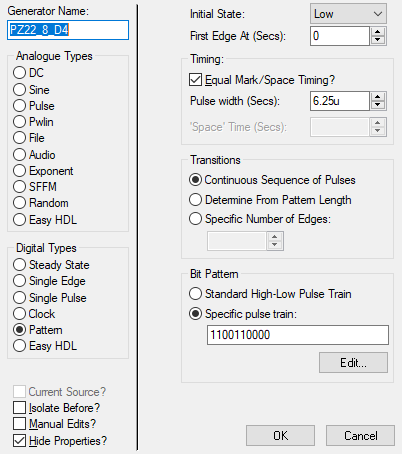
\includegraphics[width=0.45\textwidth]{41}}}
		\hspace{5px}
		\subfloat[ ]{{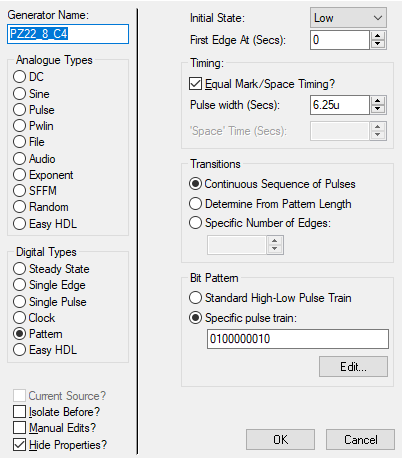
\includegraphics[width=0.45\textwidth]{42}}}
	\end{figure}

	\section*{Схема 5}	
	\begin{figure}[H]
		\centering
		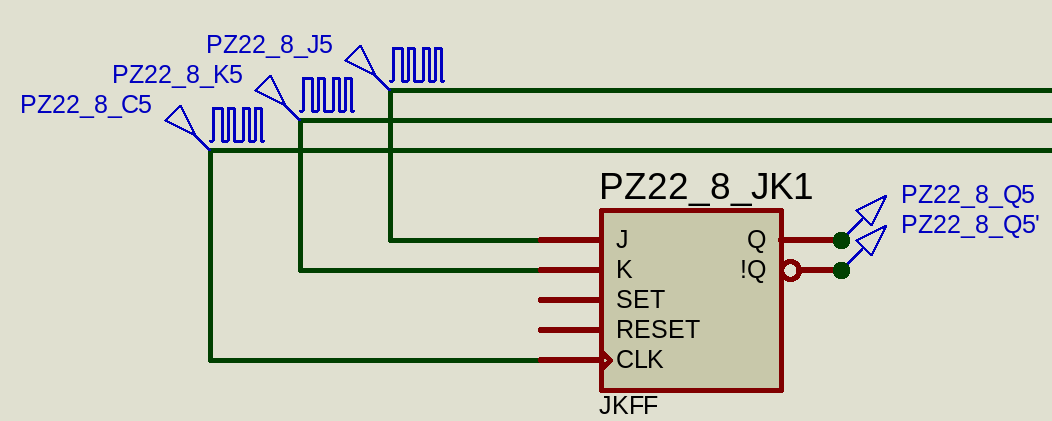
\includegraphics[scale=0.25]{s5}	
		\caption{Схема 5}
	\end{figure}
	
	\begin{figure}[H]
		\centering
		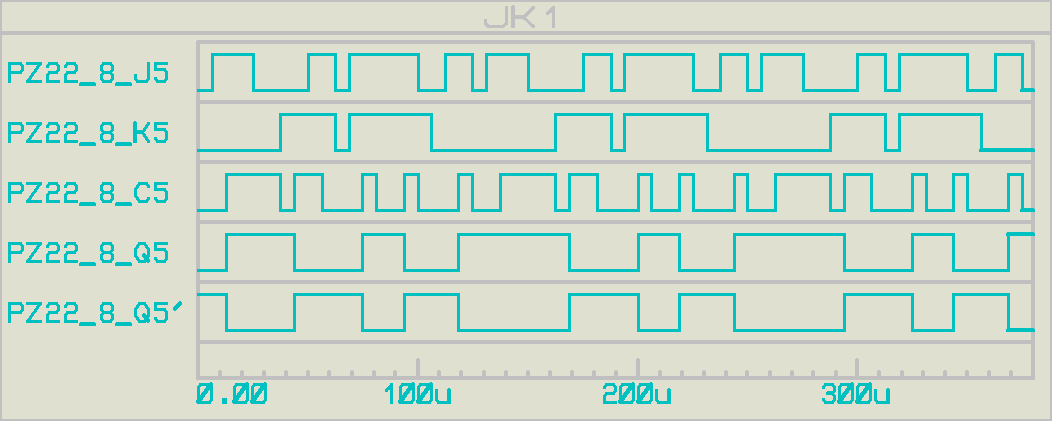
\includegraphics[scale=0.25]{g5}	
		\caption{Графік до схеми 5}
	\end{figure}

	\section*{Генератори до схеми 5}
	\begin{figure}[H]
		\centering
		\subfloat[ ]{{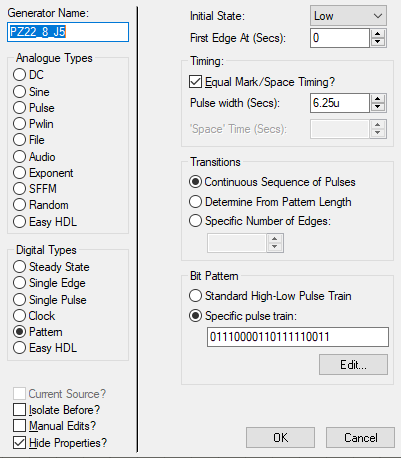
\includegraphics[width=0.45\textwidth]{51}}}
		\hspace{5px}
		\subfloat[ ]{{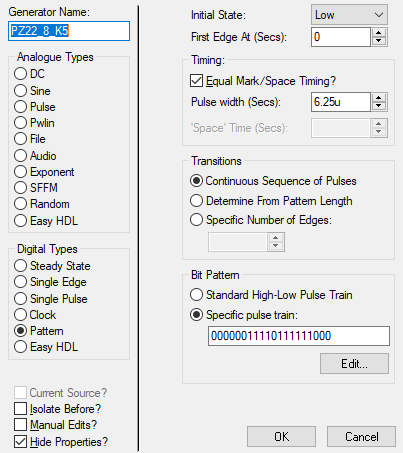
\includegraphics[width=0.45\textwidth]{52}}}
		
		\subfloat[ ]{{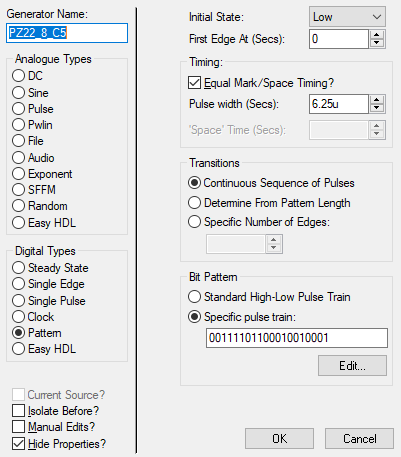
\includegraphics[width=0.45\textwidth]{53}}}
	\end{figure}

	\section*{Схема 6}	
	\begin{figure}[H]
		\centering
		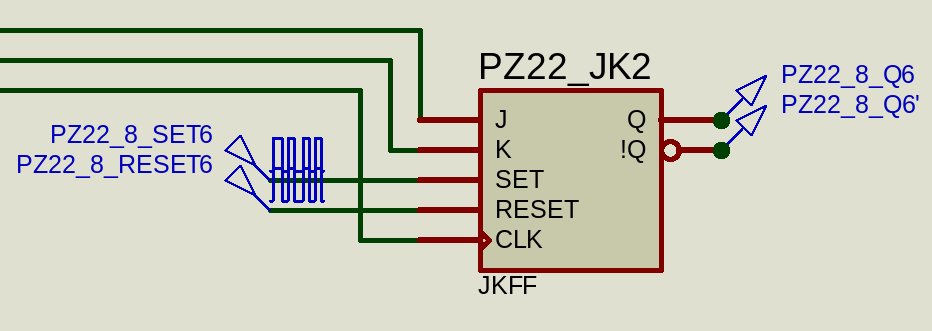
\includegraphics[scale=0.25]{s6}	
		\caption{Схема 6}
	\end{figure}
	
	\begin{figure}[H]
		\centering
		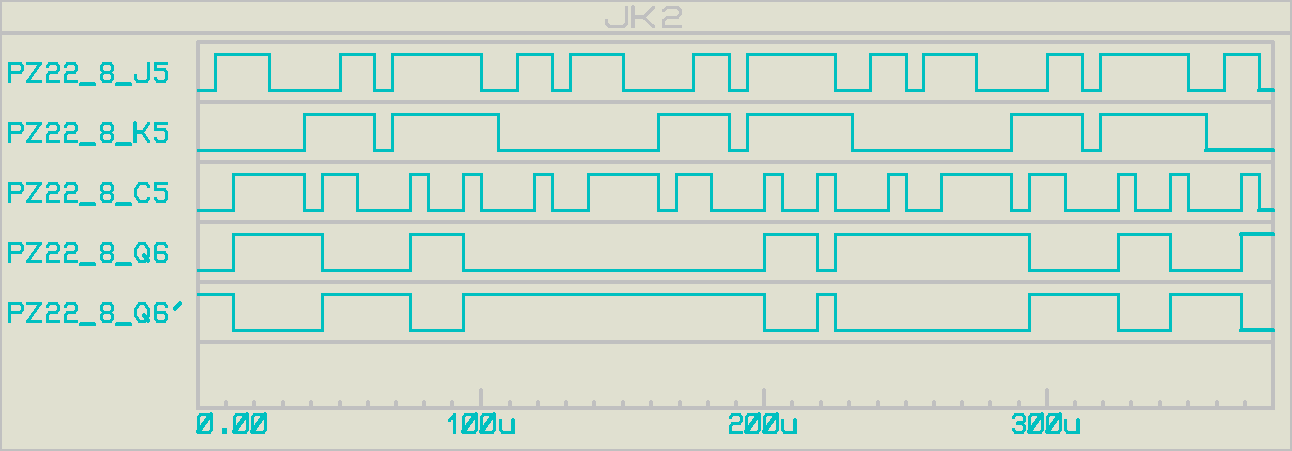
\includegraphics[scale=0.25]{g6}	
		\caption{Графік до схеми 6}
	\end{figure}

	\section*{Генератори до схеми 6}
	\begin{figure}[H]
		\centering
		\subfloat[ ]{{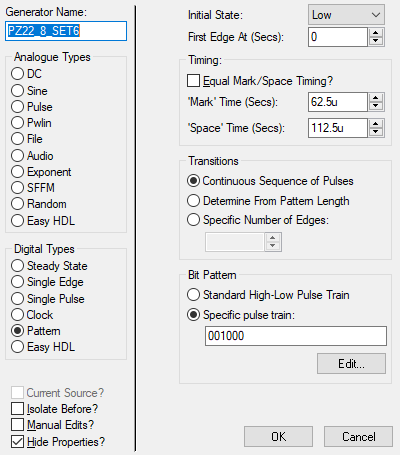
\includegraphics[width=0.45\textwidth]{61}}}
		\hspace{5px}
		\subfloat[ ]{{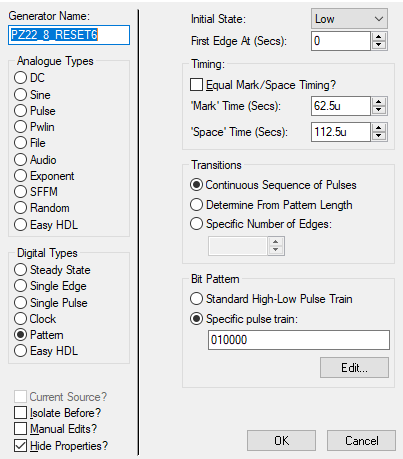
\includegraphics[width=0.45\textwidth]{62}}}
	\end{figure}

	\section*{Схема 7}	
	\begin{figure}[H]
		\centering
		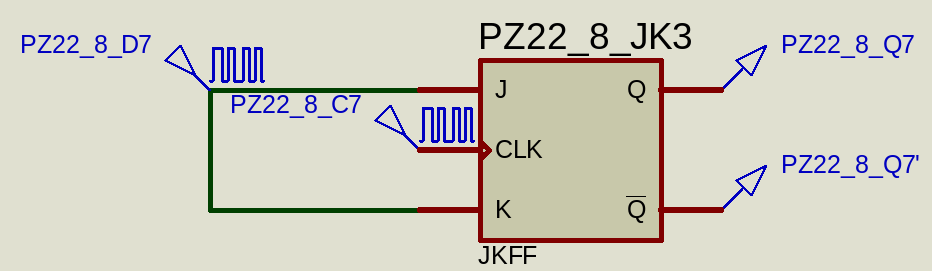
\includegraphics[scale=0.25]{s7}	
		\caption{Схема 7}
	\end{figure}
	
	\begin{figure}[H]
		\centering
		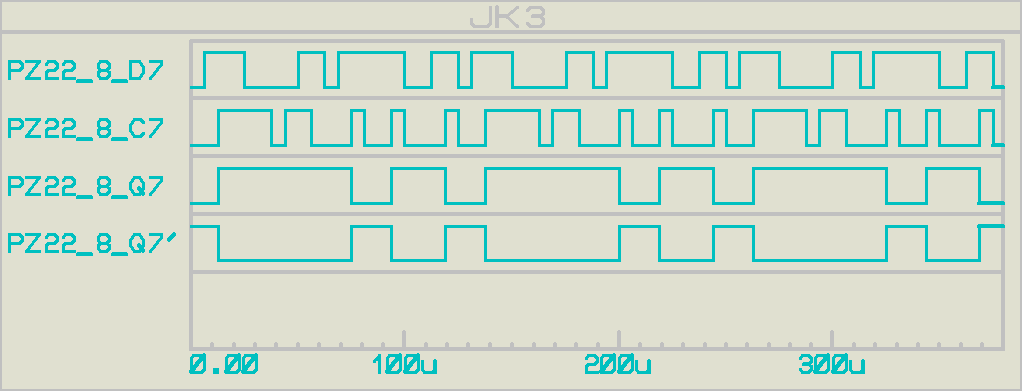
\includegraphics[scale=0.25]{g7}	
		\caption{Графік до схеми 7}
	\end{figure}

	\section*{Генератори до схеми 7}
	\begin{figure}[H]
		\centering
		\subfloat[ ]{{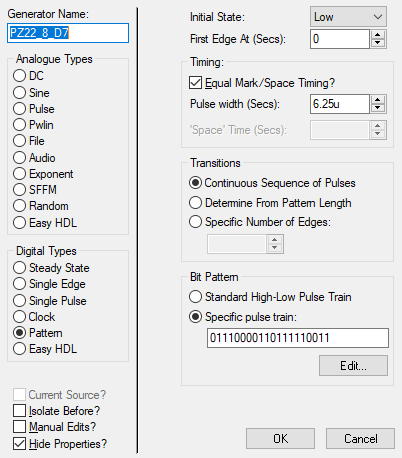
\includegraphics[width=0.45\textwidth]{71}}}
		\hspace{5px}
		\subfloat[ ]{{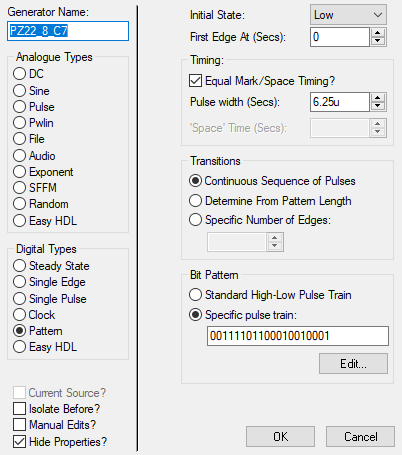
\includegraphics[width=0.45\textwidth]{72}}}
	\end{figure}

	\section*{Схема 8}	
	\begin{figure}[H]
		\centering
		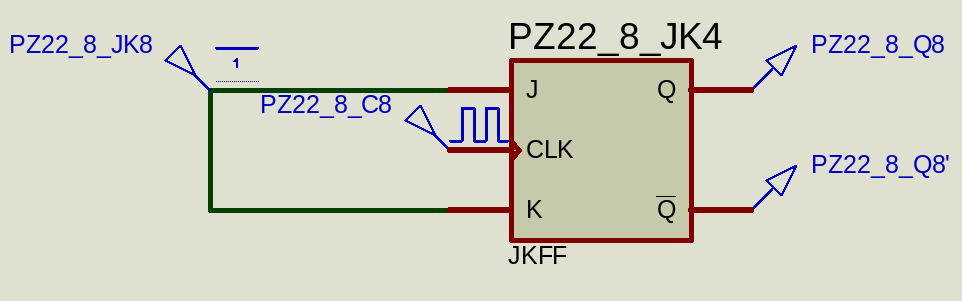
\includegraphics[scale=0.25]{s8}	
		\caption{Схема 8}
	\end{figure}
	
	\begin{figure}[H]
		\centering
		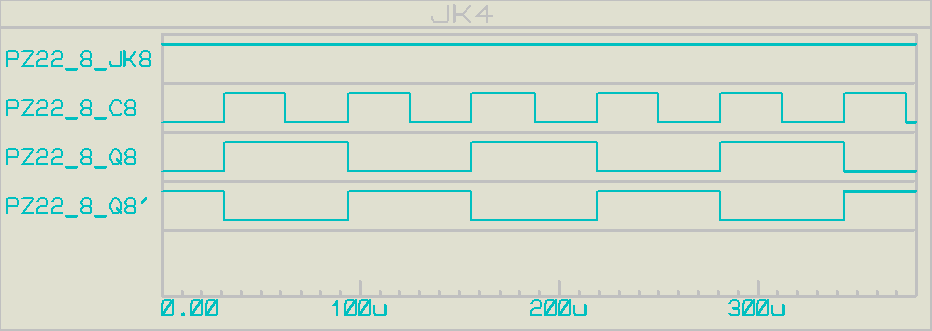
\includegraphics[scale=0.25]{g8}	
		\caption{Графік до схеми 8}
	\end{figure}

	\section*{Генератори до схеми 8}
	\begin{figure}[H]
		\centering
		\subfloat[ ]{{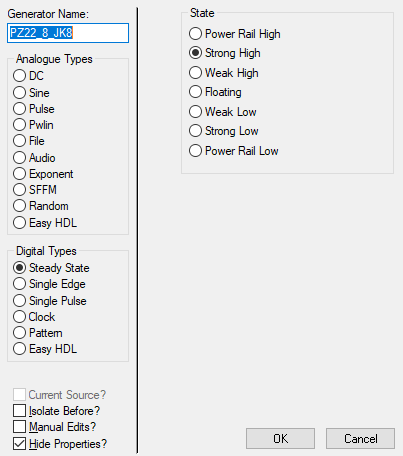
\includegraphics[width=0.45\textwidth]{81}}}
		\hspace{5px}
		\subfloat[ ]{{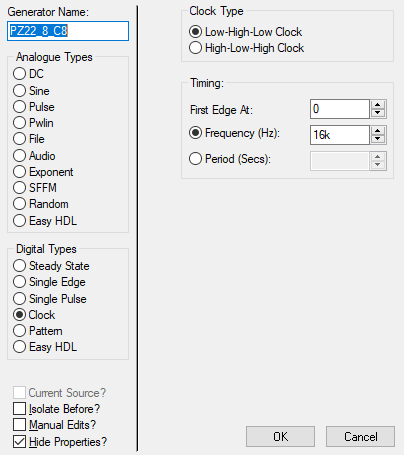
\includegraphics[width=0.45\textwidth]{82}}}
	\end{figure}

	\section*{Висновки}
	Під час виконання лабораторної роботи я закріпив практичні навики моделювання логічних схем в середовищі системи програм Proteus; поглибив знання про будову та функціонування основних типів тригерів; увів їх схеми та виконав моделювання в системі програм Proteus; дослідив на основі отриманих часових діаграм їх роботу.
	    
\end{normalsize}
\end{document}
